\clearpage
\newpage
\subsection{Local Minima}

Man erreicht das globale Minimum nur, wenn man direkt im globalem Minimum startet.
Im Endeffekt erreicht man nur in 0.059488\% der Fälle das globale Mimimum. In den restlichen Fällen landet man
entweder im lokalem Minimum (ebene Fläche im Plot), oder erreicht gar kein Minimum (Spitzen im Plot).


\begin{figure}[h!]
  \centering
  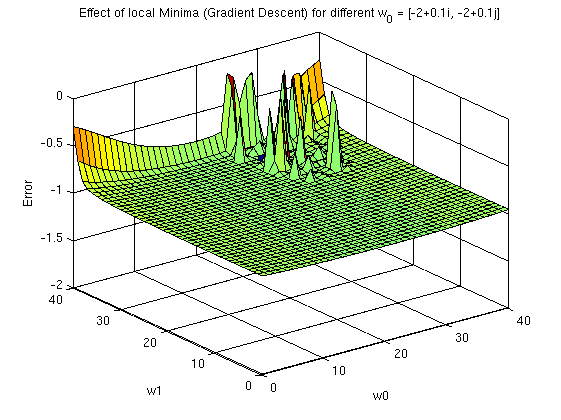
\includegraphics[width=0.8\textwidth]{./figures/214/minf.png}
  \caption{Einfluss von $\vect{w_0}$}
  \label{fig:minf}
\end{figure}